\documentclass[tikz,border=8pt]{standalone}
\usepackage{amsmath}
\usetikzlibrary{arrows.meta}
\definecolor{ink}{HTML}{21352F}\definecolor{teal}{HTML}{087F7B}\definecolor{blue}{HTML}{4B77A8}
\begin{document}
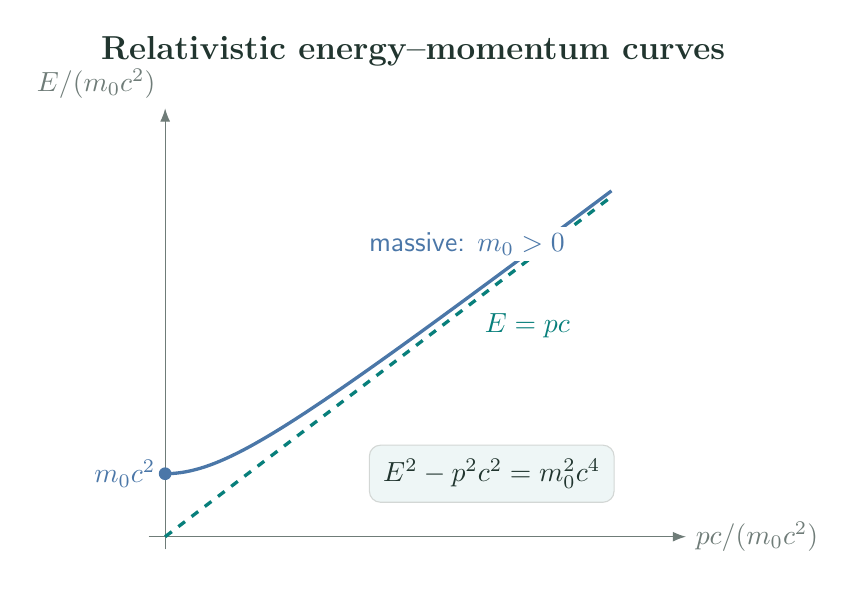
\begin{tikzpicture}[font=\sffamily,text=ink,>=Latex,x=1.05cm,y=.8cm]
  \node[font=\bfseries\large] at (3.0,7.7) {Relativistic energy--momentum curves};
  \draw[->,ink!65] (-.2,0)--(6.3,0) node[right] {$pc/(m_0c^2)$};
  \draw[->,ink!65] (0,-.2)--(0,6.8) node[above left] {$E/(m_0c^2)$};
  \draw[blue,very thick,domain=0:5.4,samples=120,smooth,variable=\x]
    plot ({\x},{sqrt(1+\x*\x)});
  \draw[teal,very thick,dashed,domain=0:5.4] plot (\x,\x);
  \node[blue,fill=white,inner sep=2pt] at (3.65,4.65) {massive: $m_0>0$};
  \node[teal,anchor=west] at (3.75,3.35) {$E=pc$};
  \fill[blue] (0,1) circle (2.3pt) node[left] {$m_0c^2$};
  \node[draw=ink!20,fill=teal!7,rounded corners=4pt,inner sep=5pt] at (3.95,1.0)
    {$E^2-p^2c^2=m_0^2c^4$};
\end{tikzpicture}
\end{document}
